\documentclass{article}
\usepackage{setup}
\begin{document}

\section*{Propositional Logic}
\subsection{Definitions}

\begin{itemize}
\item Implication: When P is true, Q must be true. False implies true.
\item $P \implies Q \equiv \neg P \lor Q$
\item If $\sigma$ is an assignment and $\varphi$ is a formula, then $\sigma \models \varphi$ (sigma satisfies phi) means $\varphi$ is true under assignment $\sigma$.
\item A formula $\varphi$ is satisfiable if there exists an assignment $\sigma$ such that $\sigma \models \varphi$. Otherwise, we say it's unsatisfiable.
\item A formula is valid (aka a tautology) if for every assignment $\sigma$, $\sigma \models \varphi$.
\item Two formulas $\varphi$ and $\psi$ are logically equivalent, denoted $\varphi \equiv \psi$, if for every assignment $\sigma$, $\sigma \models \varphi$ iff $\sigma \models \psi$.
\item Formulas $\varphi$ and $\psi$ are equisatisfiable if $\varphi$ is satisfiable iff $\psi$ is satisfiable.
\end{itemize}

\subsection{The Boolean Satisfiability Problem (SAT)}
\begin{itemize}
\item Given a propositional formula $\varphi$, is $\varphi$ satisfiable?
\item Example: System M with input x and output y and an input-output specification $\varphi(x, y)$. If we can encode the computation of M as a formula $\psi_m(x,y)$ such that this formula holds iff y is the output of M on input x ($\psi_m$ is called the input-output relation or transition relation of M), then we can decide whether M satisfies $\varphi$ for all inputs using this formula: \[\chi = \psi_m(x, y) \land \neg \varphi(x, y)\] The formula is satisfiable iff $M\not\models \varphi$, ie there is some input x such that M violates $\varphi$ on that input. So to verify M, we can check if $\chi$ is unsatisfiable.
\item Usually when we refer to SAT, we are referring to the CNF-SAT problem, where the input formula is in conjunctive normal form (CNF).
\item A formula is in CNF if it is a conjunction of clauses, where each clause is a disjunction (OR) of literals, and a literal is either a variable or the negation of a variable. Example: \[(x_1 \lor \neg x_2 \lor x_3) \land (\neg x_1 \lor x_4) \land (x_2 \lor x_3 \lor \neg x_4)
\]
\item The top level operator must be an AND.
\item Any formula can be converted to CNF.
\item A useful transformation is the Tseitin transformation, which converts any formula $\varphi$ to an equisatisfiable CNF formula $\psi$ in linear time. The idea is to introduce a new variable for each subformula of $\varphi$ and add clauses that enforce the equivalence between the new variable and the subformula. Example: \begin{align*}
\varphi = \neg(x\lor y)\lor(\neg z\land x) \\
\text{List the cases for the clause (gate) (call the output the clause u):} \\
x\implies \neg u \\
y\implies \neg u \\
\neg x \land \neg y \implies u \\
\text{Using demorgans law, we can rewrite these as:} \\
\neg x \lor \neg u \\
\neg y \lor \neg u \\
x \lor y \lor u\\
\text{AND them all together to represent the first gate!} \\
(\neg x \lor \neg u) \land (\neg y \lor \neg u) \land (x \lor y \lor u)
\end{align*}
These three clauses uniquely determine u given values for x and y (among satisfying assignments). Repeating this for every gate in the circuit gives a set of clauses encoding how the whole circuit works. Then add one more clause asserting that the output wire is true. Now any satisfying assignment of the original formula can be extended to one satisfying the new formula, and conversely any satisfying assignment of the new formula satisfies the original.
\item Since there is 1 gate per boolean operator, and a constant number of clauses per gate, the new CNF formula has size linear in the size of the original formula.
\item Disjunctive Normal Form (DNF) is the dual of CNF, where the top level operator is OR and each cube is an AND of literals. Example: \[(x_1 \land \neg x_2 \land x_3) \lor (\neg x_1 \land x_4) \lor (x_2 \land x_3 \land \neg x_4)\]
\item DNF is always satisfiable unless every cube is contradictory (eg $x_1 \land \neg x_1$).
\item SAT is solvable in linear time for DNF.
\item There is no efficient way to convert an arbitrary formula to DNF.
\end{itemize}

\subsection{Binary Decision Diagrams (BDDs)}

\begin{itemize}
\item It's a representation of boolean functions as graphs that allows varius operations (in particular, satisfiability) to be done efficiently but is more compact than a truth table.
\item A BDD is a directed acyclic graph (DAG) with: \begin{itemize}
    \item A designated root node
    \item Leaf nodes will be labeled true or false
    \item Internal nodes will be labeled with a variable and have two outgoing edges, one for the case where the variable is true and one for false.
\end{itemize}
\item The BDD for iff looks like:
\begin{center}
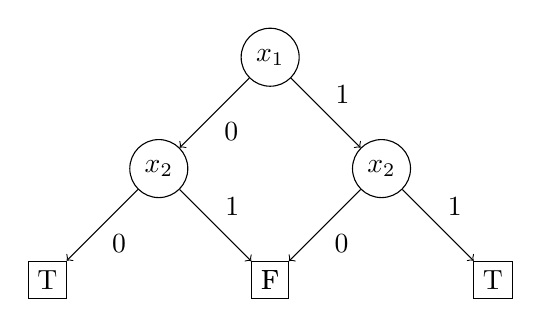
\begin{tikzpicture}[node distance=2cm, auto]
    \node[circle, draw] (x1) {$x_1$};
    \node[circle, draw, below left of=x1] (x2) {$x_2$};
    \node[circle, draw, below right of=x1] (x3) {$x_2$};
    \node[rectangle, draw, below left of=x2] (t) {T};
    \node[rectangle, draw, below right of=x2] (f) {F};
    \node[rectangle, draw, below left of=x3] (f2) {F};
    \node[rectangle, draw, below right of=x3] (t2) {T};
    \draw[->] (x1) -- node {0} (x2);
    \draw[->] (x1) -- node {1} (x3);
    \draw[->] (x2) -- node {0} (t);
    \draw[->] (x2) -- node {1} (f);
    \draw[->] (x3) -- node {0} (f2);
    \draw[->] (x3) -- node {1} (t2);
\end{tikzpicture}
\end{center}
\item Given a variable assignment, follow the corresponding edges until you reach a leaf. The value of the function is the label of the leaf.
\item Every boolean function can be represented by a BDD.
\end{itemize}

\subsection*{Reduced Ordered BDDs (ROBDDs)}
\begin{itemize}
    \item Ordered: The variables must be accessed according to a specified order along every branch of the BDD. Skipping is okay, but you cannot repeat them. An example BDD that is not ordered:
    \begin{center}
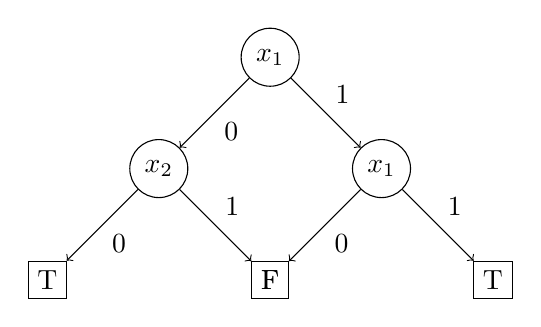
\begin{tikzpicture}[node distance=2cm, auto]
    \node[circle, draw] (x1) {$x_1$};
    \node[circle, draw, below left of=x1] (x2) {$x_2$};
    \node[circle, draw, below right of=x1] (x3) {$x_1$};
    \node[rectangle, draw, below left of=x2] (t) {T};
    \node[rectangle, draw, below right of=x2] (f) {F};
    \node[rectangle, draw, below left of=x3] (f2) {F};
    \node[rectangle, draw, below right of=x3] (t2) {T};
    \draw[->] (x1) -- node {0} (x2);
    \draw[->] (x1) -- node {1} (x3);
    \draw[->] (x2) -- node {0} (t);
    \draw[->] (x2) -- node {1} (f);
    \draw[->] (x3) -- node {0} (f2);
    \draw[->] (x3) -- node {1} (t2);
\end{tikzpicture}
\end{center}
    \item Reduced: No duplicate nodes/leaves or redundant nodes. A node is redundant if both its edges point to the same node.
    \item There is only one unique ROBDD for a given boolean function.
    \item You can check if two functions are equivalent by checking if their ROBDDs are identical.
    \item The size of the unique ROBDD for a given function can be very different depending on the variable ordering.
    \item How to build a ROBDD: Build a truth table, then build the fully expanded BDD, then reduce it.
    \item Second approach: Build from a formula in a recursive bottom-up manner by applying boolean operations. Given ROBDDs for formulas $\varphi$ and $\psi$, we can build the ROBDD for $\varphi \land \psi, \varphi \lor \psi, \neg \varphi$, etc.
    
    To do this, we'll use Shannon Expansion (aka Boole's Law), which expands a boolean function in terms of one of its variables. 

    $F(x,\cdots, x_n) \iff (x_1\land F(T, x_2, \cdots, x_n)) \lor (\neg x_1 \land F(F, x_2, \cdots, x_n))$

    \item $F(T, x_2,\cdots, x_n)$ is the positive cofactor of F with respect to $x_1$. Written $F_{x_1}(x_2, \cdots, x_n)$. \\$F(F, x_2, \cdots, x_n)$ is the negative cofactor of F with respect to $x_1$. Written $F_{\bar{x_1}}(x_2, \cdots, x_n)$.
    \item You can get the cofactors of a BDD by following the appropriate edges.
    \item Every node of the BDD corresponds to the cofactor of F with respect to the assignments leading to that node.
    \item The cofactors of the AND of two functions are the AND of the cofactors. E.g. \begin{align*}
    F(x, y) &= H(x, y) \land G(x, y) \\
    F_x(y) &= F(T, y) = H(T, y) \land G(T, y) = H_x(y) \land G_x(y) \\
    F_{\bar{x}}(y) &= F(F, y) = H(F, y) \land G(F, y) = H_{\bar{x}}(y) \land G_{\bar{x}}(y)
    \end{align*}
    It's the same for OR, NOT, etc.
    \item Extisential quantification: $\exists x_1.\varphi(x_1, \cdots, x_n) \iff \varphi(T, x_2, \cdots, x_n) \lor \varphi(F, x_2, \cdots, x_n)$
    \item Universal quantification: $\forall x_1.\varphi(x_1, \cdots, x_n) \iff \varphi(T, x_2, \cdots, x_n) \land \varphi(F, x_2, \cdots, x_n)$
    \item There are boolean functions with $n$ variables whose ROBDDs (even with the best variable ordering) have size exponential in n.
    \item Idea: Counting argument. There are $2^{2^n}$ distinct boolean functions on n variables, but fewer BDDs with less than exponential nodes.
\end{itemize}
\subsection*{Queries on BDDs}
\begin{itemize}
\item Does a given assignment/input satisfy hte formula? (Linear, simply plug into the BDD).
\item You can check satisfiability and validity in constant time. Simply check if the ROBDD is just a single true or false leaf.
\item Are two formulas equivalent? (Linear, check if the ROBDDs are identical).
\item How many satisfying assignments are there? Idea: think about all paths from the root to the true leaf.
\end{itemize}

\end{document}